\appendix
\chapter{Code source BSO}
\begin{figure}[H]
	\centering
	\includegraphics[width=\textwidth]{images/Annex/BSO/BSOSearch.png}
	\caption{Algorithme de recherche BSO générique}
\end{figure}

\begin{figure}[H]
	\centering
	\includegraphics[width=\textwidth]{images/Annex/BSO/tabuSearch.png}
	\caption{Algorithme de recherche tabou générique}
\end{figure}

\begin{figure}[H]
	\centering
	\includegraphics[width=\textwidth]{images/Annex/BSO/danceHeap.png}
	\caption{Structure de Dance en tant que Tas}
\end{figure}

\begin{figure}[H]
	\centering
	\includegraphics[width=\textwidth]{images/Annex/BSO/beeAbstract.png}
	\caption{Schéma d'une abeille générique}
\end{figure}


%\begin{figure}[H]
%	\centering
%	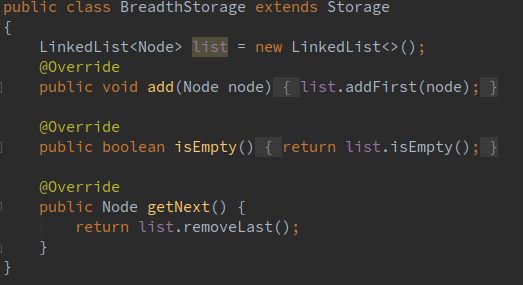
\includegraphics[width=\textwidth]{images/imgs/BFSstorage.png}
%	\caption{Gestion de open en largeur d'abord}
%\end{figure}

%\begin{figure}[H]
%	\centering
%	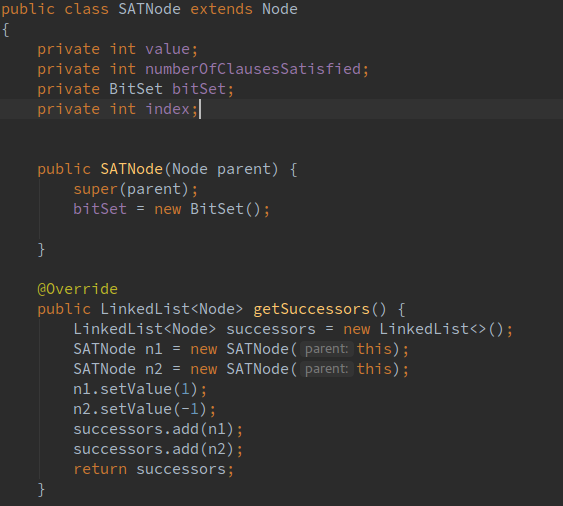
\includegraphics[width=\textwidth]{images/imgs/nodeStruct.png}
%	\caption{Structure d'un noeud dans l'arborescence}
%\end{figure}

%\begin{figure}[H]
%	\centering
%	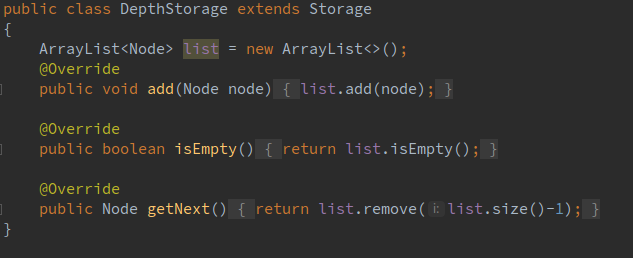
\includegraphics[width=\textwidth]{images/imgs/DFSStorage.png}
%	\caption{Gestion de open par profondeur d'abord}
%\end{figure}
%
%\begin{figure}[H]
%	\centering
%	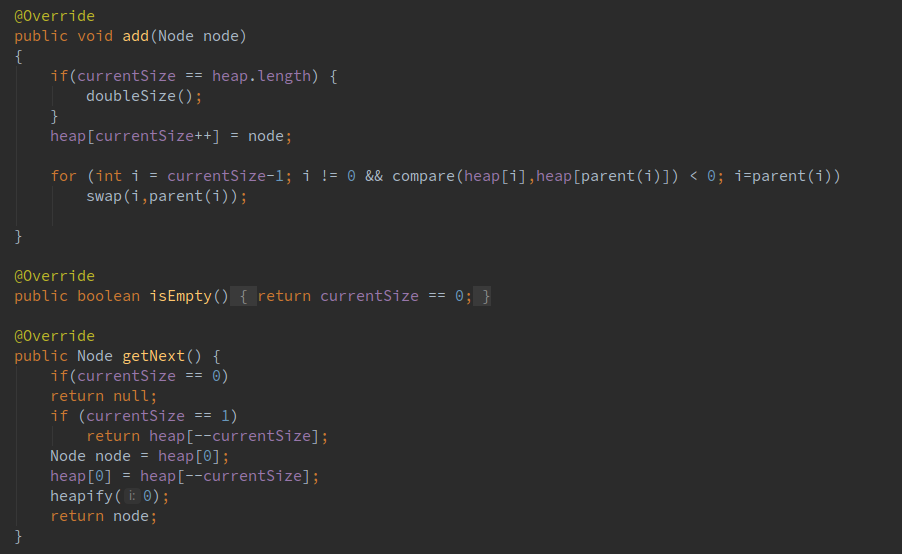
\includegraphics[width=\textwidth]{images/imgs/heapStorage.png}
%	\caption{Gestion de open en tant que tas}
%\end{figure}
%
%\begin{figure}[H]
%	\centering
%	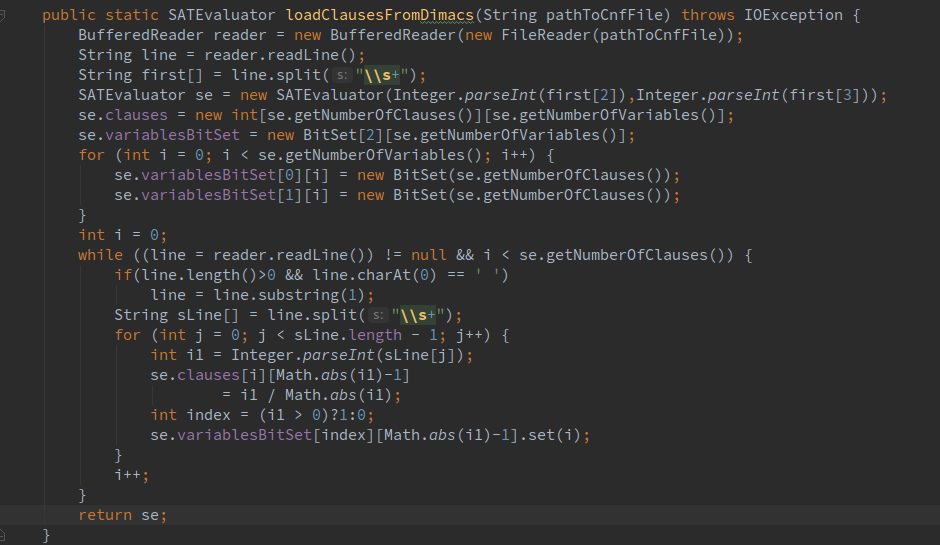
\includegraphics[width=\textwidth]{images/imgs/loadFromDimacs.png}
%	\caption{Chargement de l'instance depuis le fichier benchmark}
%\end{figure}
\chapter{Code source ACO}

\begin{figure}[H]
	\centering
	\includegraphics[width=\textwidth]{images/Annex/ACO/ACSabstract.png}
	\caption{Algorithme de recherche ACS générique}
\end{figure}

\begin{figure}[H]
	\centering
	\includegraphics[width=\textwidth]{images/Annex/ACO/ACSonline.png}
	\caption{Algorithme de recherche AS générique}
\end{figure}

\begin{figure}[H]
	\centering
	\includegraphics[width=\textwidth]{images/Annex/ACO/antAbstract.png}
	\caption{Schéma d'une fourmi générique}
\end{figure}

\begin{figure}[H]
	\centering
	\includegraphics[width=\textwidth]{images/Annex/ACO/ACSconstruct.png}
	\caption{Algorithme de construction par une fourmi ACS}
\end{figure}

\begin{figure}[H]
	\centering
	\includegraphics[width=\textwidth]{images/Annex/ACO/ASconstruct.png}
	\caption{Algorithme de construction par une fourmi AS}
\end{figure}

\begin{figure}[H]
	\centering
	\includegraphics[width=\textwidth]{images/Annex/ACO/ACSonline.png}
	\caption{Mise à jour en-ligne ACS}
\end{figure}

\begin{figure}[H]
	\centering
	\includegraphics[width=\textwidth]{images/Annex/ACO/ASonline.png}
	\caption{Mise à jour en-ligne AS}
\end{figure}

\begin{figure}[H]
	\centering
	\includegraphics[width=\textwidth]{images/Annex/ACO/pheromonsAbstract.png}
	\caption{Schéma générique de la phéromone}
\end{figure}

\begin{figure}[H]
	\centering
	\includegraphics[width=\textwidth]{images/Annex/ACO/getProba.png}
	\caption{Calcul de $P_{i,j}$}
\end{figure}

\begin{figure}[H]
	\centering
	\includegraphics[width=\textwidth]{images/Annex/ACO/pherHeur.png}
	\caption{Calcul du taux de phéromone}
\end{figure}

\begin{figure}[H]
	\centering
	\includegraphics[width=\textwidth]{images/Annex/ACO/deltaTi.png}
	\caption{Calcul du taux de phéromone a être déposé sur un litéral}
\end{figure}